\documentclass[12pt,ngerman,]{book}
\usepackage{lmodern}
\usepackage{amssymb,amsmath}
\usepackage{ifxetex,ifluatex}
\usepackage{fixltx2e} % provides \textsubscript
\ifnum 0\ifxetex 1\fi\ifluatex 1\fi=0 % if pdftex
  \usepackage[T1]{fontenc}
  \usepackage[utf8]{inputenc}
\else % if luatex or xelatex
  \ifxetex
    \usepackage{mathspec}
  \else
    \usepackage{fontspec}
  \fi
  \defaultfontfeatures{Ligatures=TeX,Scale=MatchLowercase}
\fi
% use upquote if available, for straight quotes in verbatim environments
\IfFileExists{upquote.sty}{\usepackage{upquote}}{}
% use microtype if available
\IfFileExists{microtype.sty}{%
\usepackage{microtype}
\UseMicrotypeSet[protrusion]{basicmath} % disable protrusion for tt fonts
}{}
\usepackage[margin=1in]{geometry}
\usepackage{hyperref}
\PassOptionsToPackage{usenames,dvipsnames}{color} % color is loaded by hyperref
\hypersetup{unicode=true,
            pdftitle={Praxis der Datenanalyse ENTWURF},
            pdfauthor={Sebastian Sauer. Mit Beiträgen von Oliver Gansser, Matthias Gehrke und Karsten Lübke},
            colorlinks=true,
            linkcolor=Maroon,
            citecolor=Blue,
            urlcolor=Blue,
            breaklinks=true}
\urlstyle{same}  % don't use monospace font for urls
\ifnum 0\ifxetex 1\fi\ifluatex 1\fi=0 % if pdftex
  \usepackage[shorthands=off,main=ngerman]{babel}
\else
  \usepackage{polyglossia}
  \setmainlanguage[]{german}
\fi
\usepackage{longtable,booktabs}
\usepackage{graphicx,grffile}
\makeatletter
\def\maxwidth{\ifdim\Gin@nat@width>\linewidth\linewidth\else\Gin@nat@width\fi}
\def\maxheight{\ifdim\Gin@nat@height>\textheight\textheight\else\Gin@nat@height\fi}
\makeatother
% Scale images if necessary, so that they will not overflow the page
% margins by default, and it is still possible to overwrite the defaults
% using explicit options in \includegraphics[width, height, ...]{}
\setkeys{Gin}{width=\maxwidth,height=\maxheight,keepaspectratio}
\IfFileExists{parskip.sty}{%
\usepackage{parskip}
}{% else
\setlength{\parindent}{0pt}
\setlength{\parskip}{6pt plus 2pt minus 1pt}
}
\setlength{\emergencystretch}{3em}  % prevent overfull lines
\providecommand{\tightlist}{%
  \setlength{\itemsep}{0pt}\setlength{\parskip}{0pt}}
\setcounter{secnumdepth}{5}
% Redefines (sub)paragraphs to behave more like sections
\ifx\paragraph\undefined\else
\let\oldparagraph\paragraph
\renewcommand{\paragraph}[1]{\oldparagraph{#1}\mbox{}}
\fi
\ifx\subparagraph\undefined\else
\let\oldsubparagraph\subparagraph
\renewcommand{\subparagraph}[1]{\oldsubparagraph{#1}\mbox{}}
\fi

%%% Use protect on footnotes to avoid problems with footnotes in titles
\let\rmarkdownfootnote\footnote%
\def\footnote{\protect\rmarkdownfootnote}

%%% Change title format to be more compact
\usepackage{titling}

% Create subtitle command for use in maketitle
\newcommand{\subtitle}[1]{
  \posttitle{
    \begin{center}\large#1\end{center}
    }
}

\setlength{\droptitle}{-2em}
  \title{Praxis der Datenanalyse ENTWURF}
  \pretitle{\vspace{\droptitle}\centering\huge}
  \posttitle{\par}
\subtitle{Skript zum Modul}
  \author{Sebastian Sauer. Mit Beiträgen von Oliver Gansser, Matthias Gehrke und
Karsten Lübke}
  \preauthor{\centering\large\emph}
  \postauthor{\par}
  \predate{\centering\large\emph}
  \postdate{\par}
  \date{19 June, 2017}

\usepackage{booktabs}
\usepackage{longtable}
\usepackage[bf,singlelinecheck=off]{caption}

%ses:
\pagestyle{headings}

%\setmainfont[UprightFeatures={SmallCapsFont=AlegreyaSC-Regular}]{Alegreya}

\usepackage{framed,color}
\definecolor{shadecolor}{RGB}{248,248,248}

\renewcommand{\textfraction}{0.05}
\renewcommand{\topfraction}{0.8}
\renewcommand{\bottomfraction}{0.8}
\renewcommand{\floatpagefraction}{0.75}

%\renewenvironment{quote}{\begin{VF}}{\end{VF}}
\let\oldhref\href
\renewcommand{\href}[2]{#2\footnote{\url{#1}}}

\ifxetex
  \usepackage{letltxmacro}
  \setlength{\XeTeXLinkMargin}{1pt}
  \LetLtxMacro\SavedIncludeGraphics\includegraphics
  \def\includegraphics#1#{% #1 catches optional stuff (star/opt. arg.)
    \IncludeGraphicsAux{#1}%
  }%
  \newcommand*{\IncludeGraphicsAux}[2]{%
    \XeTeXLinkBox{%
      \SavedIncludeGraphics#1{#2}%
    }%
  }%
\fi

% Hier müsste noch das Chapter mit rein! Sonst gibt es Das nicht in der Ausgabe!
% Daher habe ich das auskommentiert! (NM)
%\renewcommand{\thesection}{\arabic{section}}  % ses


\makeatletter
\newenvironment{kframe}{%
\medskip{}
\setlength{\fboxsep}{.8em}
 \def\at@end@of@kframe{}%
 \ifinner\ifhmode%
  \def\at@end@of@kframe{\end{minipage}}%
  \begin{minipage}{\columnwidth}%
 \fi\fi%
 \def\FrameCommand##1{\hskip\@totalleftmargin \hskip-\fboxsep
 \colorbox{shadecolor}{##1}\hskip-\fboxsep
     % There is no \\@totalrightmargin, so:
     \hskip-\linewidth \hskip-\@totalleftmargin \hskip\columnwidth}%
 \MakeFramed {\advance\hsize-\width
   \@totalleftmargin\z@ \linewidth\hsize
   \@setminipage}}%
 {\par\unskip\endMakeFramed%
 \at@end@of@kframe}
\makeatother

\renewenvironment{Shaded}{\begin{kframe}}{\end{kframe}}

\newenvironment{rmdblock}[1]
  {
  \begin{itemize}
  \renewcommand{\labelitemi}{
    \raisebox{-.7\height}[0pt][0pt]{
      {\setkeys{Gin}{width=3em,keepaspectratio}\includegraphics{images/icons/#1}}
    }
  }
  \setlength{\fboxsep}{1em}
  \begin{kframe}
  \item
  }
  {
  \end{kframe}
  \end{itemize}
  }
\newenvironment{rmdnote}
  {\begin{rmdblock}{note}}
  {\end{rmdblock}}
\newenvironment{rmdcaution}
  {\begin{rmdblock}{caution}}
  {\end{rmdblock}}
\newenvironment{rmdimportant}
  {\begin{rmdblock}{important}}
  {\end{rmdblock}}
\newenvironment{rmdtip}
  {\begin{rmdblock}{tip}}
  {\end{rmdblock}}
\newenvironment{rmdwarning}
  {\begin{rmdblock}{warning}}
  {\end{rmdblock}}
\newenvironment{rmdpseudocode}
  {\begin{rmdblock}{pseudocode}}
  {\end{rmdblock}}
\newenvironment{rmdexercises}
  {\begin{rmdblock}{exercises}}
  {\end{rmdblock}}
\newenvironment{rmdlove}
  {\begin{rmdblock}{love}}
  {\end{rmdblock}}

\usepackage{makeidx}  % ses
\makeindex  % ses

\urlstyle{tt}

\usepackage{amsthm}
\makeatletter
\def\thm@space@setup{%
  \thm@preskip=8pt plus 2pt minus 4pt
  \thm@postskip=\thm@preskip
}


%NM:
\def\@makechapterhead#1{%
  \vspace*{50\p@}%
  {\parindent \z@ \raggedright \normalfont
  \ifnum \c@secnumdepth >\m@ne
    \if@mainmatter
        \huge\scshape\bfseries\scshape \@chapapp\space \thechapter
        \par\nobreak
        \vskip 20\p@
    \fi
  \fi
  \interlinepenalty\@M
  \Huge \scshape\bfseries\scshape #1\par\nobreak
  \vskip 40\p@
}}

\makeatother


% NM: Zu einem frontmatter gehört auch ein mainmatter, appendix und backmatter! ;-) - Habe ich daher mal eingefügt!
\frontmatter

\begin{document}
\maketitle

{
\hypersetup{linkcolor=black}
\setcounter{tocdepth}{2}
\tableofcontents
}
\listoftables
\listoffigures
\newpage

\setcounter{chapter}{0}\chapter{Vorwort}

\begin{center}
\includegraphics[width=0.7\linewidth]{images/icons/OER_Logo_201706_gruen} \end{center}

\begin{center}
\includegraphics[width=0.1\linewidth]{images/licence} \end{center}

Statistik heute; was ist das? Sicherlich haben sich die Schwerpunkte von
``gestern'' zu ``heute'' verschoben. Wenig überraschend spielt der
Computer eine immer größere Rolle; die Daten werden vielseitiger und
massiger. Entsprechend sind neue Verfahren nötig - und vorhanden, in
Teilen - um auf diese neue Situation einzugehen. Einige Verfahren werden
daher weniger wichtig, z.B. der p-Wert oder der t-Test. Allerdings wird
vielfach, zumeist, noch die Verfahren gelehrt und verwendet, die für die
erste Hälfte des 20. Jahrhunderts entwickelt wurden. Eine Zeit, in der
kleine Daten, ohne Hilfe von Computern und basierend auf einer kleinen
Theoriefamilie im Rampenlicht standen {[}@cobb2007introductory{]}. Die
Zeiten haben sich geändert!

\begin{center}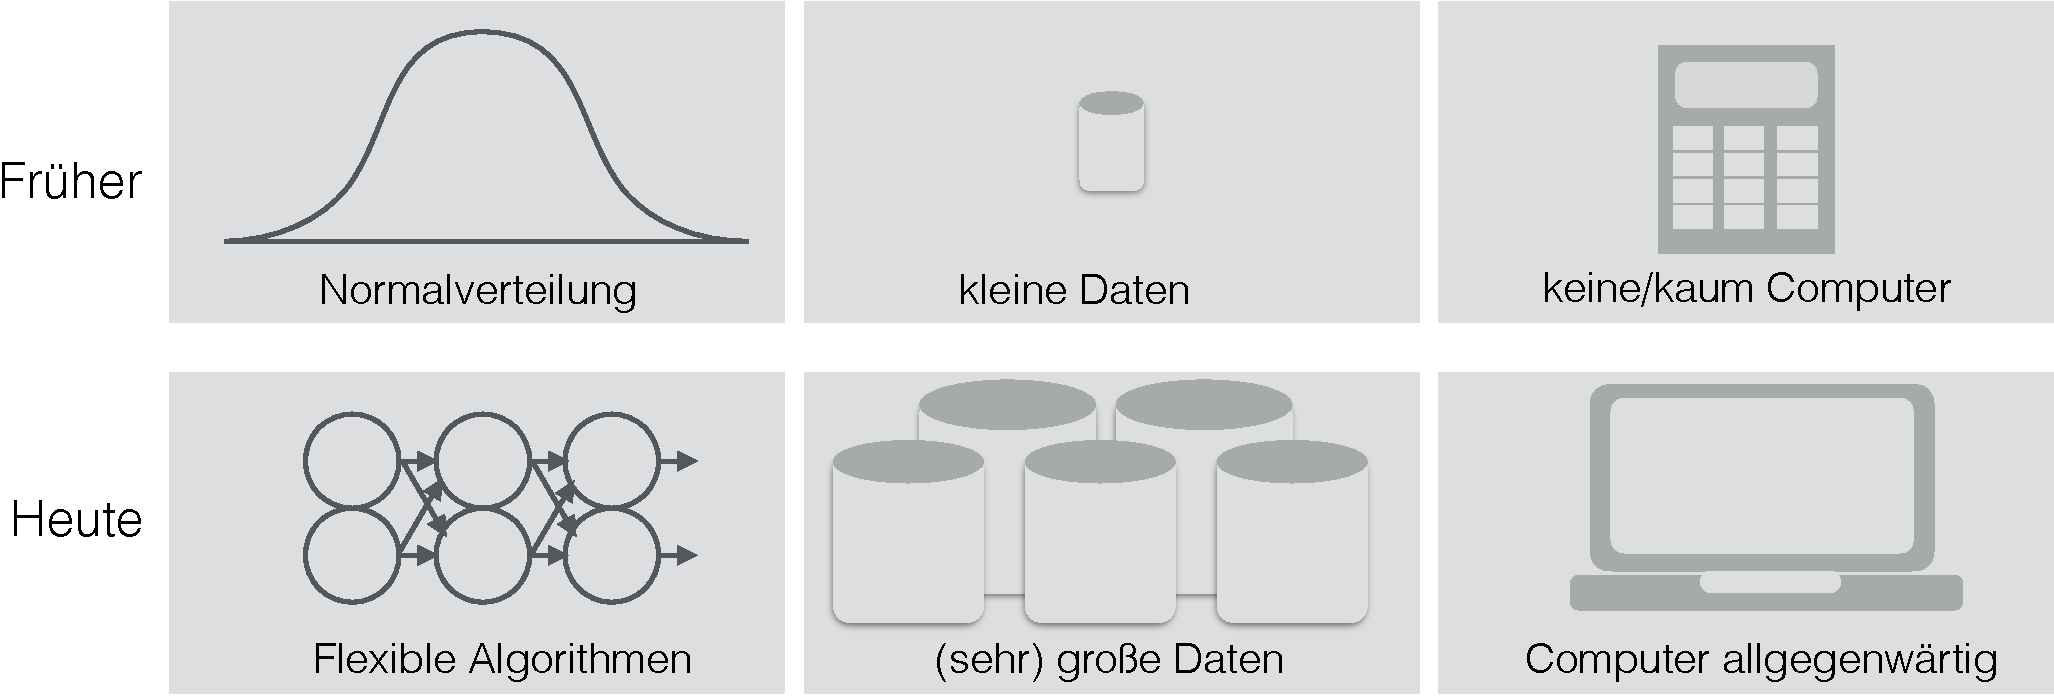
\includegraphics[width=0.7\linewidth]{images/vorwort/Forschung_frueher_heute} \end{center}

Zu Themen, die heute zu den dynamischten Gebieten der Datenanalyse
gehören, die aber früher keine große Rolle spielten, gehören
{[}@hardin2015data{]}:

\begin{itemize}
\tightlist
\item
  Nutzung von Datenbanken und anderen Data Warehouses
\item
  Daten aus dem Internet automatisch einlesen (``scraping'')
\item
  Genanalysen mit Tausenden von Variablen
\item
  Gesichtserkennung
\end{itemize}

Sie werden in diesem Kurs einige praktische Aspekte der modernen
Datenanalyse lernen. Ziel ist es, Sie - in Grundzügen - mit der Art und
Weise vertraut zu machen, wie angewandte Statistik bei führenden
Organisationen und Praktikern verwendet wird\footnote{Statistiker, die
  dabei als Vorbild Pate standen sind: Roger D. Peng:
  \url{http://www.biostat.jhsph.edu/~rpeng/}, Hadley Wickham:
  \url{http://hadley.nz}, Jennifer Bryan:
  \url{https://github.com/jennybc}}.

Es ist ein Grundlagenkurs; das didaktische Konzept beruht auf einem
induktiven, intuitiven Lehr-Lern-Ansatz. Formeln und mathematische
Hintergründe such man meist vergebens (tja).

Im Gegensatz zu anderen Statistik-Büchern steht hier die Umsetzung mit R
stark im Vordergrund. Dies hat pragmatische Gründe: Möchte man Daten
einer statistischen Analyse unterziehen, so muss man sie zumeist erst
aufbereiten; oft mühselig aufbereiten. Selten kann man den Luxus
genießen, einfach ``nur'', nach Herzenslust sozusagen, ein Feuerwerk an
multivariater Statistik abzubrennen. Zuvor gilt es, die Daten
aufzubereiten, umzuformen, zu prüfen und zusammenzufassen. Diesem Teil
ist hier recht ausführlich Rechnung getragen.

``Statistical thinking'' sollte, so eine verbreitete Idee, im Zentrum
oder als Ziel einer Statistik-Ausbildung stehen
{[}@wild1999statistical{]}. Es ist die Hoffnung der Autoren dieses
Skripts, dass das praktische Arbeiten (im Gegensatz zu einer
theoretischen Fokus) zur Entwicklung einer Kompetenz im statistischen
Denken beiträgt.

Außerdem spielt in diesem Kurs die Visualisierung von Daten eine große
Rolle. Zum einen könnte der Grund einfach sein, dass Diagramme
ansprechen und gefallen (einigen Menschen). Zum anderen bieten Diagramme
bei umfangreichen Daten Einsichten, die sonst leicht wortwörtlich
überersehen würden.

\begin{quote}
Dieser Kurs zielt auf die praktischen Aspekte der Analyse von Daten ab:
``wie mache ich es?''; mathematische und philosophische Hintergründe
werden vernachlässigt bzw. auf einschlägige Literatur verwiesen.
\end{quote}

Dieses Skript ist publiziert unter
\href{https://creativecommons.org/licenses/by-nc-sa/3.0/de/}{CC-BY-NC-SA
3.0 DE}.

\begin{center}
\includegraphics[width=0.1\linewidth]{images/licence} \end{center}

Sebastian Sauer

\begin{center}\rule{0.5\linewidth}{\linethickness}\end{center}

\textbf{Herausgeber: FOM Hochschule für Oekonomie \& Management
gemeinnützige GmbH}

Dieses Skript dient als Begleitmaterial zum Modul ``Praxis der
Datenanalyse'' des Masterstudiengangs ``Wirtschaftspsychologie \&
Consulting'' der FOM Hochschule für Oekonomie \& Management.

FOM. Die Hochschule. Für Berufstätige. Die mit bundesweit über 42.000
Studierenden größte private Hochschule Deutschlands führt seit 1993
Studiengang für Berufstätige durch, die einen staatlich und
international anerkannten Hochschulabschluss (Bachelor/Master) erlangen
wollen. Weitere Informationen finden Sie unter
\textless{}www.fom.de\textgreater{}

\printindex

\backmatter


\end{document}
